\chapter{Requirements and Existing Solutions}

\section{Usage Scenarios}
\label{usecases}
\subsection{Asking for Help}
Having the possibility to ask for help is a vital part of the working culture in many knowledge driven
businesses, so collaboration and the sharing of ideas are a major factor in the company guidelines
of SinnerSchrader. The application is supposed to act as a central repository for knowledge and contacts,
enabling employees to find someone who can help in order to answer questions and find solutions to domain-specific problems.

\subsection{Finding Potential Team Members}
Team managers constantly face the problem of reassembling parts of their teams, forming new teams for new projects, and
disbanding teams whose projects have ended. As there is no unified source of information about all employees at SinnerSchrader, managers often
do not find the most suitable team member to fill an open position because they simply do not know each other yet.
This tool will give managers the opportunity to search the entirety of SinnerSchrader's workforce and find the most suitable one
meeting all requirements of the open position, thus making collocating teams easier and more efficient.

\newpage

\section{Collecting the Required Features}
\label{interviewquestions}
As shown in \ref{usecases}, the application is supposed to provide help for two target audiences: project managers staffing their teams, and employees looking for help with a certain problem.
The actual features the system should include have been collected by the \textit{Flow Team}, a group of project managers who coordinate and monitor project team staffing and personnel development at SinnerSchrader. This team also supervises the development of the skills management application. To validate that the requirements asked by them reflect the end users' needs, and to obtain a better impression thereof, semi-structured interviews have been conducted. In addition to collecting the asked persons' general expectations, the interviews aimed to give answers to these concrete questions:
\begin{itemize}
	\item What should be the range of the scale used to measure knowledge and motivation?
	\item Should the overall experience of the employees be captured by the system?
	\item Should the system differentiate between short-term and long-term motivation?
	\item Should users be able to rate their colleagues' skills?
	\item Should the system be able to automatically form project teams?
\end{itemize}

\subsection{Interview Procedure}
The interviews consist of a ten-minute-long\footnote{The actual timeframe may vary depending on the interviewee's answers.} open discussion between the interviewer and the interviewees, so that in the event of the interviewee giving an extraordinaire answer or bringing up a new idea, the interviewer may ask for further explanations. The questions listed in \ref{interviewquestions} will provide a guideline to structure the interviews. Before the interview, the interviewees have been informed about the procedure, the personal data that will be collected for the interview and the purpose of its collection, and had to give their written consent (see \ref{consentform}).
In order to extract all information from the interviewees' answers, audio recordings have been taped during the interviews.

\newpage

\subsection{Interviewees}
As described, there are three main groups of stakeholders regarding the application: the Flow Team that supervises its development, project managers who search for new team members, and \textit{regular} employees looking for help. For each of these groups, one representative has been interviewed:
\begin{itemize}
	\item Ms. Spranger\\
	Ms. Spranger is the Product Owner in the developemt team and part of the Flow Team for which she will speak.
	\item Mr. Warnholz\\
	Mr. Warnholz is a project manager and has many years of experience with various teams at SinnerSchrader. He frequently searches for
	employees fitting into specific project teams and will represent the project managers' point of view.
	\item Mr. Gruber\\
	Mr. Gruber is a backend developer and supervisor of one of SinnerSchrader's domain-specific teams. As he worked on multiple projects that
	use drastically different technology stacks and processes, he is familiar with the problem of having to look for colleagues that can help with a specific problem.
\end{itemize}
In contrast to Ms. Spranger, Mr. Warnholz and Mr. Gruber have not been in contact with the development of the skills management application, so that their opinions should not be influenced by internal decisions made about the tool's design.

\subsection{Results}
The interview recordings have been transcribed (see \ref{transcripts}) to extract information about the interviewees' opinions to decide whether or not the respective feature should be included in the application, and if so, how it should be designed.

\subsubsection{General Expectations}
Popular features requested by the interviewees include the ability to see how motivated employees are regarding specific skills in order to increase employee satisfaction and to deduce a certain employee's development of interest. Furthermore, one of the most desired features is that project managers get a tool to find suitable members for their teams. Qualitative factors the interviewees requested are that the tool is easy to use and that the interface is reduced to the most important components.

\newpage

\subsubsection{Scale}
\label{scale_definition}
When asked for a rough estimate of how the scale on which knowledge and motivation will be measured should be designed, all interviewees replied that they prefer a simple scale between four and six values. Mr. Gruber and Mr. Warnholz proposed to use five step \textit{Likert-Style Items}.
% Since those items are based on the idea of estimating the distance to a neutral element in both directions (e.g. better or worse), this type of scale is not applicable for the measurement of knowledge.
The chosen approach will include a scale of four items for both types of values:
\begin{center}
\begin{tabular}{c|c}
	Knowledge & Motivation \\
	\hline
	novice & uninterested\\
	basic knowledge & indifferent\\
	advanced knowledge & somewhat interested\\
	expert & highly interested\\
\end{tabular}
\end{center}


\subsubsection{Overall Experience}
All interviewees agree that the overall experience of the employees should not be included in the search function because the skill-specific experience is significantly more meaningful in this context. The general grade of experience that is reflected by the employee's title (e.g. \textit{Junior}, \textit{Intermediate} or \textit{Senior}) should be shown in the result list but it must not influence the search or rating.

\subsubsection{Duration of Motivation}
Regarding the question whether the duration of a will, that is how long the interest in a specific skill will persist, should be captured in the system, the interviewees agree that this ought not be the case. The system is supposed to present a snapshot of the present situation and should not be used for long term assumptions. Another important factor stated by the interviewees is that forecasts about one's motivation will be highly inaccurate.

\subsubsection{Peer Rating}
\label{peerrating}
All of the interviewees answered that they do not want employees to be able to rate each other's skills because they fear that subjective impressions might blur the professional view leading to a heavy influence of sympathy on the ratings. Furthermore, the works council prohibits the introduction of such a feature (see \ref{legal_concerns}) because multiple employees raised concerns about this kind of functionality and wish it not to be included. To respect their demands, users of the application will not be able to rate someone other than themselves.

\subsubsection{Generating Teams}
The application will not save which projects each employee works on or has previously worked on, because this information is managed by another internal service which will not be replaced by this application. This data would then have to be updated in both systems manually. Under this condition, no interviewee wants the application to automatically compose project teams. Reasons that have been mentioned are that maintaining the same data in two systems\footnote{The project management system and the skills management application} is impractical, that this task is too complex to be automated, and that composing complete teams is not a popular use case for it. Project teams at SinnerSchrader grow organically, so it is much more common for project managers to look for one single potential member to add to their team instead of composing a completely new one. Based on these insights, the application will not be able to compose teams.

\section{Workflows for Collecting Data}

The application will give employees the opportunity to provide information about their personal knowledge regarding their skills.
Furthermore, they can assign a will value for every skill that describes if they prefer
doing the implicitly linked activity or working with the tool described by said skill. That is, people can define what they want to do and what tasks they would like to refuse.\\
With employees continually enlarging their knowledge and their fields of interest shifting towards new technologies, tools, or even
functional divisions, providing data about their skills and preference only once will lead to the system being filled with obsolete
information. The quality of the search results and suggestions heavily relies on the fidelity and volume of the underlying data about the employees, hence keeping that information up to date is crucial to the performance of the application.

\subsection{Biannual Feedback Meetings}
Every employee has biannual meetings with their supervisor to exchange
bidirectional feedback, define personal goals, and negotiate possible changes of salary.
Part of the feedback given by the employee are subjects they learned or enhanced their knowledge about, and newly developed interests. These insights are documented and registered in the employee's personnel file.
The aforementioned meeting will be the regular occasion for supervisors and employees to refine the data saved in the application and to add
newly gained skills to it. The supervisor is advised to address discrepancies between the employee's estimations of skills and their own one to accommodate the human factors of self-perception. A case study performed by Beck indicates that this approach to
collect information about the employees' skills generates a sufficient amount of data to run such a system \cite{beck}.

\subsection{Data Maintenance}
Employees and supervisors are encouraged to be in rich contact with each other in order to deliver continuous feedback
about the individual person's needs, impediments, and the status of their current projects.
As a result, supervisors can identify appropriate moments for reevaluating the skills and preferences saved in the application and notify the employee.\\
For example, according to Tuckman's team development model, the so called \textit{adjourning} phase of a project is an occasion for ``recognition of individual achievements and reflection on how far the team has come'' \cite[P. 3]{Wilson} and thus is a convenient chance to add new skills acquired during the project and to refine the existing data.\\
In contrast to the supervisor, the application will not be able to find the best situations to notify employees to maintain their skill profile, so sending automatic notifications will not be nearly as effective as being reminded by the supervisor. Furthermore, according to the \textit{Direct Marketing Association (UK)}\footnote{https://dma.org.uk/}, only
about one in five automatically generated e-mails will be opened \cite{mailrep}, which reflects SinnerSchrader's
experiences with email reminders. Those facts justify the decision that the system will not send any notification to its users.

\subsubsection{Intrinsic Motivations}
In addition to the mentioned reasons for employees to provide data about their skills which are all extrinsic motivations,
there also are intrinsic motivations to do so. Being motivated intrinsically is defined as ``doing something because it is inherently interesting or enjoyable'' \cite{RYAN200054}. As people are motivated to focus on tasks they fancy, they are also motivated to voluntarily keep an eye on the quality of the data that is used to determine the tasks they will have to perform.

\newpage

\section{Requirements}
Based on the Flow Team's demands and the data collected in the interviews, functional and non-functional requirements for to application have been composed.

\label{requirements}
\subsection{Functional Requirements}
\begin{itemize}
 	\item Accessible to all Employees\\
	Every employee must be able to use the application regardless of their equipment or preferred operating system.
	\item User Profiles \\
	Anyone can see another user’s profile consisting of basic information about the user such as name, location, e-mail and personal skills. Personal skills are composed of a name, a skill level, and a will level. The last two describe the employee's knowledge and motivation regarding the respective skill.
	\item Provide/Edit skills\\
	Users can add new skills from a pool of predefined skills to their own profile. Already added skills can be edited and removed from the profile.
	\item Search\\
	A search function can be used to find people who have added one or more specific skills to their profile. When searching for multiple skills, only persons matching all of them will be displayed.
	\begin{itemize}
		\item Ranking\\
			By default, the search results' order will be defined by a score aggregating the individual employee's skill levels, will levels and grade of specialization in the searched skills. The specialization is defined as the difference between the employee's average levels in the searched skills and in the unsearched skills.
		\item Sorting\\
			The users are able to sort the search results not only by said score
			but also by skill and will level.
	\item Provide Additional Information\\
			Employees are able to add comments to their profile to give extra information about working hours, special contracts, certificates they own, etc.
	\end{itemize}
	\item Management of Known Skills\\
	New skills can be added to the set of known skills in the application. Existing skills can be edited and removed. Users' personal skills are automatically updated when a skill has been edited, so that the integrity of the users' profiles is maintained at all times.
\end{itemize}

\newpage

\subsection{Non-Functional Requirements}
\begin{itemize}
	\item Device Types\\
		Even tough smartphones are gaining a constantly increasing share in terms of total internet traffic \cite{allthemobile},
		the application will be optimized for desktop use. Every employee has permanent access to their computer and uses it
		for their work, so it can be assumed that the very same machines will be used to access the skill management application.
	\item Browsers\\
		Every employee is allowed and encouraged to install their favorite software on their personal computer, so nearly every web browser can be found.
		The application should run on \textit{Google Chrome}\footnote{https://www.google.com/chrome/browser/desktop/index.html}, \textit{Mozilla Firefox}\footnote{https://www.mozilla.org/en-US/firefox/products/} and \textit{Safari}\footnote{http://www.apple.com/lae/safari/} in their latest versions. \textit{Internet Explorer}\footnote{https://www.microsoft.com/en-us/download/internet-explorer.aspx} and \textit{Edge}\footnote{https://www.microsoft.com/en-us/windows/microsoft-edge} will not be supported. Explanations on these decisions are given by Strecker \cite{strecker}.
	\item Scalability\\
		SinnerSchrader has 459 full-time employees \cite{quartalsbericht}, so the application will be designed for approximately 500 users. In the event of rapid growth in the userbase, e.g. due to the opening of another office, the system will have to scale up to handle the larger number of users.
	\item Load/Response Times\\
		According to \textit{Google's} RAIL model, a website needs to respond to the user's input within 100ms to offer a fluent user experience; the triggered action should be finished within one second after the user's interaction \cite{RAIL}. In the context of the application's search function, this means that the system will show the user that their input has been acknowledged within 100ms. Within one second after the submission of the search request, the result list will be rendered completely. 	\label{require_times}
\end{itemize}



\section{Commercial Solutions}
\label{commercial}
Three commercial skills management applications have been picked randomly for further examination: \textit{Skills Base}, \textit{Talent Management (engage!)} and \textit{SkillsDB Pro}.
A more detailed analysis by Lehner shows that most tools provide a spectrum of features and limitations very similar to the examined solutions \cite{Marktanalyse}, so that the selection is assumed to be representative to the market.

\subsection{Skills Base}
Skills Base\footnote{http://www.skills-base.com/} offers most of the required features, but also includes a large number of functionality SinnerSchrader does not need and is not willing to use. This includes assessments, the categorization of skills, and a role model for advanced access rights configuration.
A central aspect of the application are dashboards displaying information about the most popular skills in the organization and long term statistics. The API supports searching for multiple skills with minimum levels in knowledge and interest. Unfortunately, the application cannot be hosted by SinnerSchrader. This means the employees data would have to be stored on external infrastructure that is operated and monitored by an external company, which should be avoided due to legal reasons.
\begin{figure}[!htp]
    \centering
    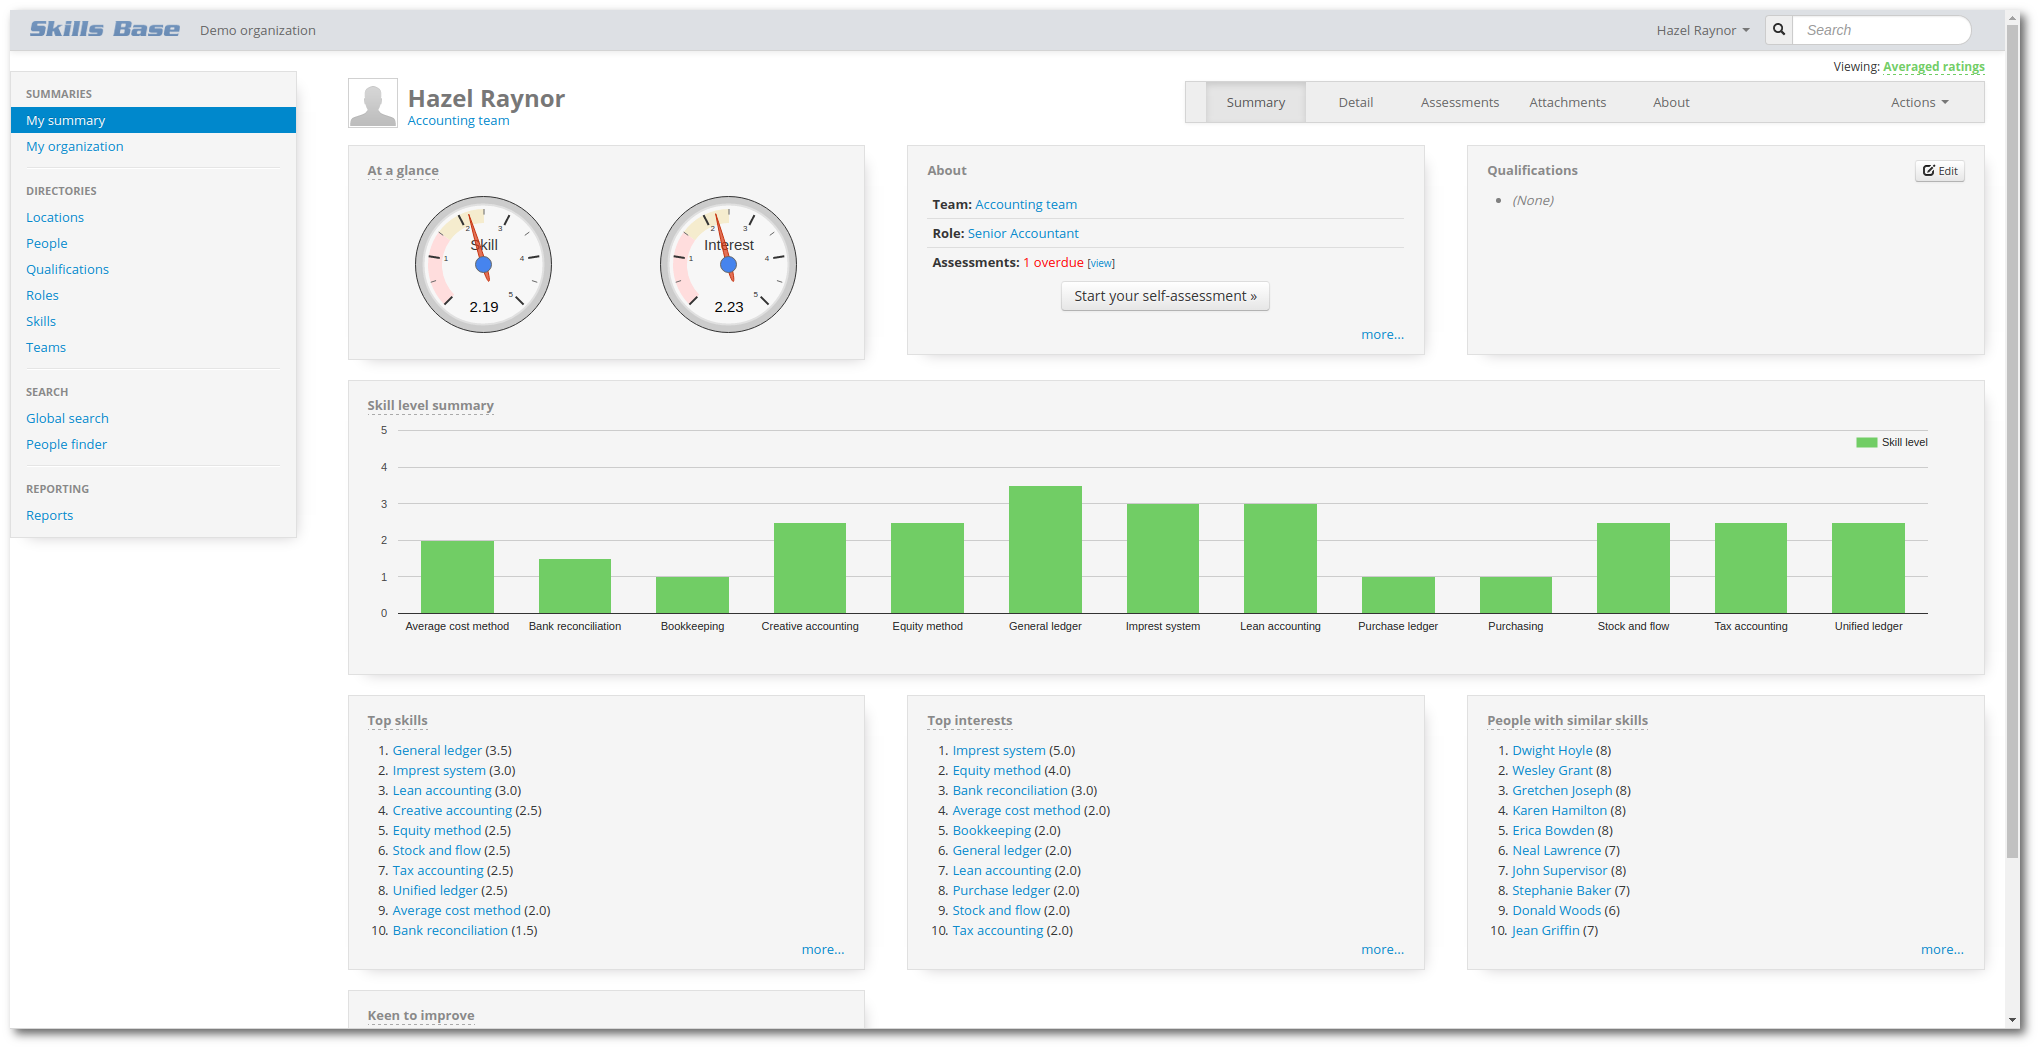
\includegraphics[width=\textwidth]{images/skillsbase-dashboard.png}
    \caption[Screenshot: SkillsBase Dashboard]{SkillsBase Dashboard (source: \textit{https://www.youtube.com/user/SkillsBase})}
    \label{fig:skillsbase_dashboard}
\end{figure}

\subsection{Talent Management (engage!)}
Talent Management\footnote{http://www.infoniqa.com/hr-software/skill-management} is a module for \textit{Infoniqa’s} management software engage!\footnote{http://www.infoniqa.com/hr-software/personalmanagement}. It offers advanced features for managers such as a powerful search function controlled via a special query language. It also includes data about the employees’ salaries, feedback protocols, and certificates, but lacks the feature to register motivation. It can only be used in combination with engage!, a complete human resources management solution including features like time tracking, e-learning, applicant management and payroll accounting.

\subsection{SkillsDB Pro}
SkillsDB Pro\footnote{http://www.skillsdbpro.com} is an application designed to serve as a database in an organization, providing an overview of every person’s personal skills and training only to themselves and their supervisor. The search function is capable of searching for multiple skills combined with different logical operators which enables users to enter very sophisticated queries.
Not only can users provide information about their skills but supervisors can also do this with the limitation that no employee can see their supervisor's rating about themselves. Information about motivation, like in the other examined systems, cannot be captured.
Furthermore, only privileged users like supervisors can search for persons. Taking into consideration that SinnerSchrader needs a tool to enable everyone to find someone with a specific skill set, this is a serious disadvantage.
SkillsDB Pro also offers features SinnerSchrader does not intend to use including the automatic generation of project reports based on plan succession and demands for assessments.

\begin{figure}[!htp]
    \centering
    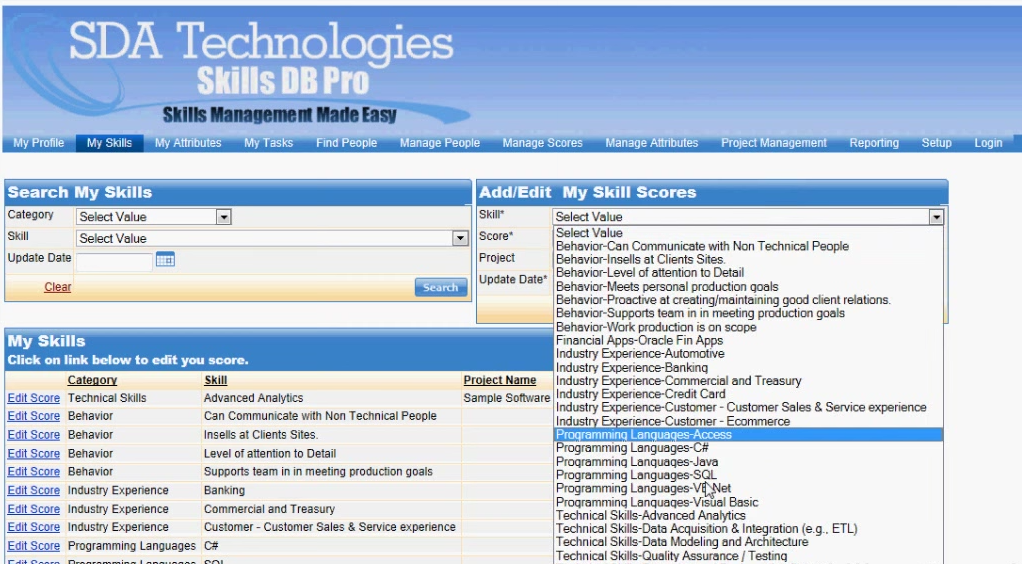
\includegraphics[width=\textwidth]{images/skillsdbpro.png}
    \caption[Screenshot: SkillsDB Pro Overview]{SkillsDB Pro Overview (source: \textit{http://skillsdbpro.com/})}
    \label{fig:talent_management}
\end{figure}

\newpage

\subsection{Conclusion}
None of the analyzed applications offer all required features, but all of them include various functions SinnerSchrader does not intend to use, which brings undesired complexity into the application.
One of the most critical features, a search function that aggregates both knowledge and motivation is not offered by any of the commercial solutions.
Furthermore, all those systems differentiate between employees and their supervisors and thus restrain transparency. The application is not supposed to be used for monitoring and rating employees, but should give employees the possibility to find each other; categorizing them into different roles would clearly defeat this purpose.

\subsubsection{Pain Point Fitness Scoring}
As shown by Canós‐Darós, motivation is a vital factor regarding any employee's performance and quality of work \cite{CanosDaros2013}.
Although motivation is a complex construct of many highly diverse dimensions, the size of the intersection of a person's interests and their duties is a key aspect to it. Assuming that every member of the company has some skills they prefer to employ over others, matching people to tasks that require the exact same abilities they are interested in employing will lead to more motivated employees and thus have a positive impact on the overall productivity.
Consequently, when searching for persons having specific skills, the application should not only take into account the employees' skills but also their preferences in order to not find the most skilled, but the best fitting one. Unfortunately, none of the examined applications provide a way to aggregate both skills and preferences into a single score indicating the overall grade of suitability of a person relative to the searched skills.
